\documentclass{standalone}
\begin{document}
\subsection{Color Quantization}
	
	Colour quantization is the process of reducing the number of colours in a digital image preserving significant information. In other words, the quantization process should not cause significant information loss in the image.  The colour quantizes image should be very close to the original image, visually as in \figurename\,\ref{fig:ColorQuantization}. 


	\begin{figure}[h!]	
		\centering
			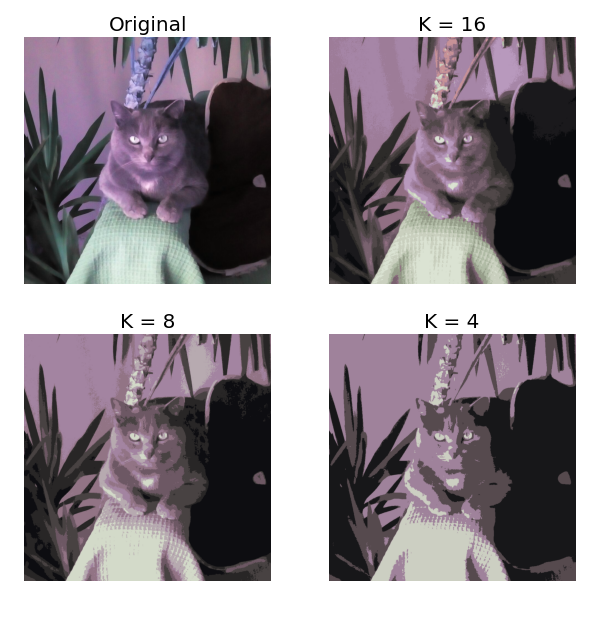
\includegraphics[scale=.3]{ColorQuantization.png}
		\caption{\textit{Colour quantized GL image. We observe the original image, a 32 colour image which looks similar to the original one, a 16 colours image and 8 colours image. The tissues are grouped by colour similarity. Reduce the colour to the number of the cluster allows pixel classification. }}\label{fig:ColorQuantization}
	\end{figure}

	Colour quantization plays an important role in many application fields such as segmentation, compression, colour texture analysis, watermarking, 
	text localization/detection, non photorealistic rendering and content-based retrieval~\cite{ART:Ozturk}.
		
	Colour quantization is used for image segmentation. To this purpose the algorithm aims to reduce the number of colours in the image to one of the different tissues, assigning a characteristic colour to each one of them. This is the case of medical image segmentation, in which each image colour represents a particular characteristic of the tissue displayed (i.e in x-ray represent$\mu$). 
	To perform this technique, different algorithms may be used to group the colours, like clustering algorithm or the principal component analysis.


	
	
	
	

	
	
\end{document}